%  A simple AAU report template.
%  2015-05-08 v. 1.2.0
%  Copyright 2010-2015 by Jesper Kjær Nielsen <jkn@es.aau.dk>
%
%  This is free software: you can redistribute it and/or modify
%  it under the terms of the GNU General Public License as published by
%  the Free Software Foundation, either version 3 of the License, or
%  (at your option) any later version.
%
%  This is distributed in the hope that it will be useful,
%  but WITHOUT ANY WARRANTY; without even the implied warranty of
%  MERCHANTABILITY or FITNESS FOR A PARTICULAR PURPOSE.  See the
%  GNU General Public License for more details.
%
%  You can find the GNU General Public License at <http://www.gnu.org/licenses/>.
%
%  A simple AAU report template.
%  2015-05-08 v. 1.2.0
%  Copyright 2010-2015 by Jesper Kjær Nielsen <jkn@es.aau.dk>
%
%  This is free software: you can redistribute it and/or modify
%  it under the terms of the GNU General Public License as published by
%  the Free Software Foundation, either version 3 of the License, or
%  (at your option) any later version.
%
%  This is distributed in the hope that it will be useful,
%  but WITHOUT ANY WARRANTY; without even the implied warranty of
%  MERCHANTABILITY or FITNESS FOR A PARTICULAR PURPOSE.  See the
%  GNU General Public License for more details.
%
%  You can find the GNU General Public License at <http://www.gnu.org/licenses/>.
%
%\documentclass[oneside]{book}
\documentclass[11pt,oneside,a4paper,openright]{report}
%%%%%%%%%%%%%%%%%%%%%%%%%%%%%%%%%%%%%%%%%%%%%%%%
% Language, Encoding and Fonts
% http://en.wikibooks.org/wiki/LaTeX/Internationalization
%%%%%%%%%%%%%%%%%%%%%%%%%%%%%%%%%%%%%%%%%%%%%%%%
% Select encoding of your inputs. Depends on
% your operating system and its default input
% encoding. Typically, you should use
%   Linux  : utf8 (most modern Linux distributions)
%            latin1 
%   Windows: ansinew
%            latin1 (works in most cases)
%   Mac    : applemac
% Notice that you can manually change the input
% encoding of your files by selecting "save as"
% an select the desired input encoding. 
\usepackage[utf8]{inputenc}
% Make latex understand and use the typographic
% rules of the language used in the document.
\usepackage[english]{babel}
% Use the palatino font
\usepackage[sc]{mathpazo}
\linespread{1.05}         % Palatino needs more leading (space between lines)
% Choose the font encoding
\usepackage[T1]{fontenc}
%%%%%%%%%%%%%%%%%%%%%%%%%%%%%%%%%%%%%%%%%%%%%%%%
% Graphics and Tables
% http://en.wikibooks.org/wiki/LaTeX/Importing_Graphics
% http://en.wikibooks.org/wiki/LaTeX/Tables
% http://en.wikibooks.org/wiki/LaTeX/Colors
%%%%%%%%%%%%%%%%%%%%%%%%%%%%%%%%%%%%%%%%%%%%%%%%
% load a colour package
\usepackage{xcolor}
\definecolor{aaublue}{RGB}{33,26,82}% dark blue
% The standard graphics inclusion package
\usepackage{graphicx}
\usepackage{float}
% Set up how figure and table captions are displayed
\usepackage{caption}
\captionsetup{%
  font=footnotesize,% set font size to footnotesize
  labelfont=bf % bold label (e.g., Figure 3.2) font
}
% Make the standard latex tables look so much better
\usepackage{array,booktabs}
% Enable the use of frames around, e.g., theorems
% The framed package is used in the example environment
\usepackage{framed}

%%%%%%%%%%%%%%%%%%%%%%%%%%%%%%%%%%%%%%%%%%%%%%%%
% Mathematics
% http://en.wikibooks.org/wiki/LaTeX/Mathematics
%%%%%%%%%%%%%%%%%%%%%%%%%%%%%%%%%%%%%%%%%%%%%%%%
% Defines new environments such as equation,
% align and split 
\usepackage{amsmath}
% Adds new math symbols
\usepackage{amssymb}
% Use theorems in your document
% The ntheorem package is also used for the example environment
% When using thmmarks, amsmath must be an option as well. Otherwise \eqref doesn't work anymore.
\usepackage[framed,amsmath,thmmarks]{ntheorem}

%%%%%%%%%%%%%%%%%%%%%%%%%%%%%%%%%%%%%%%%%%%%%%%%
% Page Layout
% http://en.wikibooks.org/wiki/LaTeX/Page_Layout
%%%%%%%%%%%%%%%%%%%%%%%%%%%%%%%%%%%%%%%%%%%%%%%%
% Change margins, papersize, etc of the document
\usepackage[
  inner=28mm,% left margin on an odd page
  outer=41mm,% right margin on an odd page
  ]{geometry}
% Modify how \chapter, \section, etc. look
% The titlesec package is very configureable
\usepackage{titlesec}
\titleformat{\chapter}[display]{\normalfont\huge\bfseries}{\chaptertitlename\ \thechapter}{20pt}{\Huge}
\titleformat*{\section}{\normalfont\Large\bfseries}
\titleformat*{\subsection}{\normalfont\large\bfseries}
\titleformat*{\subsubsection}{\normalfont\normalsize\bfseries}
%\titleformat*{\paragraph}{\normalfont\normalsize\bfseries}
%\titleformat*{\subparagraph}{\normalfont\normalsize\bfseries}

% Clear empty pages between chapters
\let\origdoublepage\cleardoublepage
\newcommand{\clearemptydoublepage}{%
  \clearpage
  {\pagestyle{empty}\origdoublepage}%
}
\let\cleardoublepage\clearemptydoublepage

% Change the headers and footers
\usepackage{fancyhdr}
\pagestyle{fancy}
\fancyhf{} %delete everything
%\renewcommand{\headrulewidth}{0pt} %remove the horizontal line in the header
%\fancyhead[RE]{\small\nouppercase\leftmark} %even page - chapter title
%\fancyhead[LO]{\small\nouppercase\rightmark} %uneven page - section title
%\fancyhead[LE,RO]{\thepage} %page number on all pages
\fancyfoot[C]{\thepage} % except the right
\renewcommand{\headrulewidth}{0pt}
%\renewcommand{\footrulewidth}{0pt}}
% Do not stretch the content of a page. Instead,
% insert white space at the bottom of the page
\raggedbottom
% Enable arithmetics with length. Useful when
% typesetting the layout.
\usepackage{calc}

%%%%%%%%%%%%%%%%%%%%%%%%%%%%%%%%%%%%%%%%%%%%%%%%
% Bibliography
% http://en.wikibooks.org/wiki/LaTeX/Bibliography_Management
%%%%%%%%%%%%%%%%%%%%%%%%%%%%%%%%%%%%%%%%%%%%%%%%
\usepackage{csquotes}
\usepackage[backend=bibtex,
  bibencoding=utf8,
  urldate=comp
  ]{biblatex}
\addbibresource{bib/mybib.bib}

%%%%%%%%%%%%%%%%%%%%%%%%%%%%%%%%%%%%%%%%%%%%%%%%
% Misc
%%%%%%%%%%%%%%%%%%%%%%%%%%%%%%%%%%%%%%%%%%%%%%%%
% Add bibliography and index to the table of
% contents
\usepackage[nottoc]{tocbibind}
% Add the command \pageref{LastPage} which refers to the
% page number of the last page
\usepackage{lastpage}
% Add todo notes in the margin of the document
\usepackage[
%  disable, %turn off todonotes
  colorinlistoftodos, %enable a coloured square in the list of todos
  textwidth=\marginparwidth, %set the width of the todonotes
  textsize=scriptsize, %size of the text in the todonotes
  ]{todonotes}

%%%%%%%%%%%%%%%%%%%%%%%%%%%%%%%%%%%%%%%%%%%%%%%%
% Hyperlinks
% http://en.wikibooks.org/wiki/LaTeX/Hyperlinks
%%%%%%%%%%%%%%%%%%%%%%%%%%%%%%%%%%%%%%%%%%%%%%%%
% Enable hyperlinks and insert info into the pdf
% file. Hypperref should be loaded as one of the 
% last packages
\usepackage{hyperref}
\hypersetup{%
	pdfpagelabels=true,%
	plainpages=false,%
	pdfauthor={Author(s)},%
	pdftitle={Title},%
	pdfsubject={Subject},%
	bookmarksnumbered=true,%
	colorlinks=false,%
	citecolor=black,%
	filecolor=black,%
	linkcolor=black,% you should probably change this to black before printing
	urlcolor=black,%
	pdfstartview=FitH%
}

\makeatletter
\def\@makechapterhead#1{%
  \vspace*{50\p@}%
  {\parindent \z@ \raggedright \normalfont
    %\ifnum \c@secnumdepth >\m@ne
    %    \huge\bfseries \@chapapp\space \thechapter
    %    \par\nobreak
    %    \vskip 20\p@
    %\fi
    \interlinepenalty \@M
    \Huge \bfseries \thechapter$.$ #1 \par \nobreak
    \vskip 40\p@
  }}
\makeatother

\graphicspath{ {figures/} }
\usepackage{dirtytalk}
\usepackage{listings}
\usepackage{color}
 
\definecolor{codegreen}{rgb}{0,0.6,0}
\definecolor{codegray}{rgb}{0.5,0.5,0.5}
\definecolor{codepurple}{rgb}{0.58,0,0.82}
\definecolor{backcolour}{rgb}{0.95,0.95,0.92}
 
\lstdefinestyle{mystyle}{
    backgroundcolor=\color{backcolour},   
    commentstyle=\color{codegreen},
    keywordstyle=\color{magenta},
    numberstyle=\tiny\color{codegray},
    stringstyle=\color{codepurple},
    basicstyle=\footnotesize,
    breakatwhitespace=false,         
    breaklines=true,                 
    captionpos=b,                    
    keepspaces=true,                 
    numbers=left,                    
    numbersep=5pt,                  
    showspaces=false,                
    showstringspaces=false,
    showtabs=false,                  
    tabsize=4
}
 
\lstset{style=mystyle}
\lstset{language=C++}

\usepackage{epigraph}

\newcommand\tab[1][0.55cm]{\hspace*{#1}}
% package inclusion and set up of the document
% see, e.g., http://en.wikibooks.org/wiki/LaTeX/Formatting#Hyphenation
% for more information on word hyphenation
\hyphenation{ex-am-ple hy-phen-a-tion short}
\hyphenation{long la-tex}% 

\begin{document}
%frontmatter
\pagestyle{empty} %disable headers and footers
\pagenumbering{arabic}
%\pagenumbering{arabic} %use arabic page numbering in the frontmatter
%  A simple AAU report template.
%  2015-05-08 v. 1.2.0
%  Copyright 2010-2015 by Jesper Kjær Nielsen <jkn@es.aau.dk>
%
%  This is free software: you can redistribute it and/or modify
%  it under the terms of the GNU General Public License as published by
%  the Free Software Foundation, either version 3 of the License, or
%  (at your option) any later version.
%
%  This is distributed in the hope that it will be useful,
%  but WITHOUT ANY WARRANTY; without even the implied warranty of
%  MERCHANTABILITY or FITNESS FOR A PARTICULAR PURPOSE.  See the
%  GNU General Public License for more details.
%
%  You can find the GNU General Public License at <http://www.gnu.org/licenses/>.
%
\pdfbookmark[0]{Front page}{label:frontpage}%
\begin{titlepage}
  \addtolength{\hoffset}{0.5\evensidemargin-0.5\oddsidemargin} %set equal margins on the frontpage - remove this line if you want default margins
  \noindent%
  \vspace{0.2cm}
  \begin{tabular}{@{}p{\textwidth}@{}}
    \toprule[2pt]
    \midrule
    \begin{center}
      \Huge{\textbf{
      Design and development of a game framework % insert your title here
      }}
    \end{center}
    \vspace{0.2cm}\\
    \midrule
    \toprule[2pt]
  \end{tabular}
  \begin{center}
  \vspace{0.4cm}
    {\large
      Hummingbird Framework \& MOGL Plugin\\
      June 22nd, 2016
    }\\
    \vfill
    \vspace{0.2cm}
    {\Large
      \begin{center}
        \textit{Author:} \\
        Alessio Linares Bernardini\\
        \textit{Director:} \\
        Guillem Godoy\\
      \end{center}
    }
  \end{center}
  \vspace{0.2cm}
  \begin{center}
  Barcelona School of Informatics\\
  Polytechnic University of Catalonia
  \end{center}
\end{titlepage}
\clearpage

\pdfbookmark[0]{Contents}{label:contents}
\pagestyle{fancy} %enable headers and footers again
\tableofcontents
\clearpage
\addcontentsline{toc}{chapter}{\tab \lstlistlistingname}
\lstlistoflistings
\cleardoublepage
%mainmatter
\setlength{\parskip}{1em}
\chapter{Preamble}\label{ch:preamble}

Through this document, the various functionalities of the resulting product, the Hummingbird 
framework, are explained with examples. For a complete description of each class and 
its methods a reference manual is included appended at the end of this document.

\chapter{Context}\label{ch:context}
My interest in game development started almost at the same time as my interest in 
programming.

First, I started experimenting with Game Maker\cite{GameMaker}, where I was able to easily make 
games by basically drag-and-dropping icons that represented changes in the state 
of the game. After a lot of trial and error and messing with its scripting language 
too, I decided to try another tool: Unity Game Engine.
Unity offered a more complex environment but it also allowed for more complex things
. I started learning it by doing tutorials and eventually made a few mini-games.

At that point I wanted to implement games in a much lower level. I wanted to understand 
the insides of how a game works. I started programming games in C++ without using 
any game developing framework or engine (only using SFML\cite{SFML} for multimedia and rendering
). The first time was very complicated, but the more games I developed, the better 
I saw a common pattern in their structure. I always had a main loop\cite{gameloop} with a game 
state update and render; some kind of object pool; some kind of input handling; and 
some kind of rendering pipeline. On the other hand, I was almost never able to reuse 
them because I like trying new technologies, libraries or methods, and most of the 
time these common structures were entangled with calls to the specific libraries 
I was using at the moment.

Eventually, I told to myself, why not implement all these functionalities once, in 
a way that is reusable for my future projects? This is where this project comes into 
place, to implement a flexible and extensible game development framework.

\chapter{State of the art}\label{ch:state_of_the_art}

The functionalities of the game framework I want to develop for this project do not 
conform a full game engine, but they are just a part of what a game engine has to 
offer. For this reason, I considered convenient to study some commercial game engines. 
There exist generic game engines and game engines specialized in specific genres. 
I focused on the generic ones, such as Unity\cite{unity3d} and Unreal Engine
\cite{unrealengine}, because one of my goals is to use it for different projects. 
Both mentioned engines use componentization for giving their actors (game objects 
in Unity) behavior and properties \cite{uecomponents}\cite{unitycomponents}. Unity 
also implements a main loop with a fixed update\cite{unitymainloop}, that is better 
for AI and physics simulations, as it provides stability and allows for simplicity
\cite{gameloop}. On the other hand it is good to render as fast as you can and 
Unity has the rendering outside of the fixed update.

They also implement some kind of resource management that allows easy access to resources 
without having multiple copies of the same. Which is a basic functionality 
for preventing filling the memory with unneeded data.

I also read the on-line book Game Programming Patterns\cite{gameprogrammingpatterns}, 
by Bob Nystrom, to get ideas and solutions to the problems I may face when implementing 
the framework.

\chapter{Formulation of the problem}\label{ch:formulation_of_the_problem}

The problem I want to solve is having to implement the same infrastructure every 
time that I make a game. That infrastructure consists of having a main loop, a pool 
of game objects (each of them possibly having different behaviors) and handling their 
data.

This infrastructure, framework, must also be flexible enough to allow me to experiment 
with new technologies (rendering libraries, networking, physics, etc.) in the future 
without requiring to change its code, making it widely easier to develop games.

\chapter{Objective}\label{ch:objective}

The goal of this project is to design and implement a game development framework that 
solves the problem described in the previous section. The framework will have solved 
the problem when it presents the functionalities listed bellow.

\begin{itemize}
\item The framework implements some basic helper classes for game development. That is, 
a way to describe transformations of objects and tools for measuring and storing intervals 
of time;
\item The framework implements a main loop with fixed update;
\item The framework handles the creation, destruction and storage of game actors. These 
actors will contain behaviors that will define its actions and properties;
\item The framework offers a way of handling resources (loading, accessing, freeing);
\item The framework will allow extending the main loop with a plug-in system. This feature 
makes possible adding a rendering pipeline, physics simulation, etc. without having 
to touch the framework code.
\end{itemize}

Finally, for demonstrating the usage of the plug-in system. This project will also 
implement a plug-in that wraps the SFML library. The SFML plug-in will implement:

\begin{itemize}
\item The resource management of textures, music, sounds, etc. using the structure offered 
by the framework;
\item An input handling system;
\item A 2D rendering pipeline using the SFML utilities.
\end{itemize}

\chapter{Scope}\label{ch:scope}

This project is part of a bigger project that consists of developing a full game engine. 
Due to time constraints the project will be limited to just the core of the game engine. 
Said core will consist of the framework that results of this project and that will 
be limited to the functionalities listed in the objectives above. For the sake of 
simplicity and avoiding possible complications, the framework spatial system will 
be limited to the 2 dimensional plane.

Moreover, the project does not consist of developing a game nor it is part of it. 
It's sole goal is to develop the game framework.

\chapter{Anatomy of a game}\label{ch:anatomy_of_a_game}

\epigraph{A video game is an electronic game that involves human interaction with 
a user interface to generate visual feedback on a video device such as a TV screen 
or computer monitor.}{Wikipedia}

The quote above is Wikipedia's definition for \textit{video game}. From it we 
can extract the various parts that form a video game:

\begin{itemize}
\item It's a game;
\item Involves human interaction (input);
\item From the input generate some feedback;
\item The feedback is visual (video).
\end{itemize}

In this document we won't tackle the topic of \textit{what makes a game a game}. Instead 
we'll focus on the other three points, which are specific to video games.

The first thing to clear up is that a video game, \textit{game} from now on for simplicity, 
consists of an input-feedback loop. If it wasn't a loop a game would only last one 
frame.

We'll call this input-feedback loop \textbf{main loop} or \textbf{game loop} and 
in its simplest form it looks like the following:

\pagebreak
\begin{lstlisting}[caption=Basic main loop.]
while (true)
{
  processInput(); // Get the human interaction
  update(); // generate the feedback
  render(); // display the feedback
}
\end{lstlisting}

This is an extremely simplified version of a game loop. More complex versions may 
include sleep time between cycles, to lower the power consumption, or include a fixed 
cycle rate, which is useful for physics and AI simulation.

\section{Actors and Scenes}

As games grow more complex, proper structuration of data becomes more important, not 
only for efficiency but mainly for easying the development process. Generally, this 
structure is given by the division of the game in \textbf{scenes} and the representation 
of the game world through \textbf{actors} (or game objects).

Scenes are the natural division of a game. A scene can be a level, a menu screen, 
etc. Usually, they set up the configuration needed for that given part of the game, 
when they start, and, when done, they handle the clean up.

Actors, on the other hand, are the objects that live in the game world. From the player 
to the rock blocking the player's path. They, as their name suggests, \textit{act} 
in the game's world simulation.

\chapter{Project implementation}\label{ch:project_implementation}

The following sections will explain the evolution of the project and the available 
classes and their jobs in the final product. Refer to the reference manual appended 
at the end of the document for a full and detailed list of all the functionalities 
of each class.

\section{Evolution of the implementation}

Throughout the development of the project the design of the framework has suffered changes. 
A few of them are explained below.

\subsection{Removal of Scene}
The initial design of the framework included a class for scenes. After a few iterations 
the Scene class felt pointless, having the only functionality of creating the required 
actors at the start, keeping track of them and finally destroying them.

This functionality can be implemented, with better results, with a plugin that does 
exactly the same. With the advantage that said plugin would be tailored to whatever 
needs the actual implementation of the game uses (p.e. scene file format).

And so, the Scene class was droped.

\subsection{Vector2 and Vector3}
Initialy there were not going to be any kind of vector class. The Transformation class 
would include all needed spatial information and that was it.

When the implementation of MOGL started, more and more the need for a way to represent 
spatial information was needed. Mainly to normalize the representation of said information, 
at one point there were sf::Vector3 and glm::vec3 in the public API of the library.

The decision was made to implement Vector2 and Vector3 in a effort to unify the spatial 
information throughout all the Hummingbird framework and MOGL plugin.

\subsection{Draw using OpenGL}
The initial plan was to make use of SFML's Drawable classes to render. At some point 
the decision was made to render the geometry directly using OpenGL so that future implementations 
of Drawables for 3D geometry were easier.

This change implied a complete refactor of the rendering pipeline, requiring the 
management of shaders and the addition of a camera.

\section{Hummingbird}

Hummingbird is the name of the base framework. In this section I'll explain how 
use the functionalities it features. The classes and methods that compose the framework 
are all contained inside the \textbf{hum} (\textbf{hum}mingbird) namespace.

For more information on each of the classes and methods check the hum namespace 
section of reference manual appended to this document.

\subsection{Game}

The Game class handles the game loop and the lifecycle of the game. To start
running a Game just call \texttt{run()} and the Game instance will enter the
following flow chart. The flow chart shows the lifecycle of a Game and the
different steps that happen through it.


\begin{figure}[H]
    \centering
    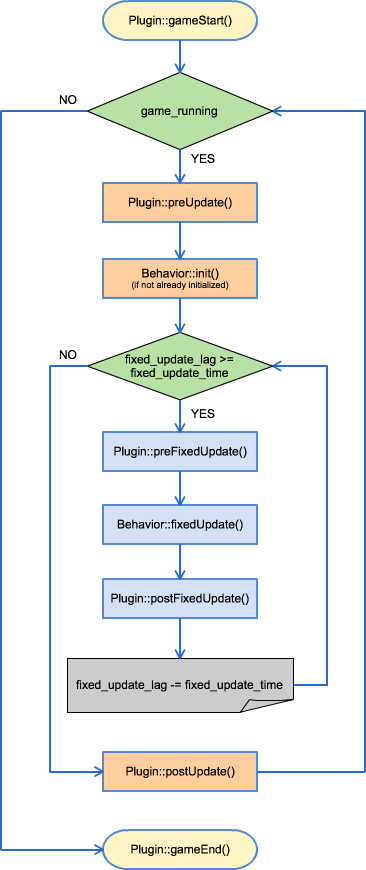
\includegraphics[width=0.5\textwidth]{game_loop}
    \caption{Game loop}
    \label{fig:game_loop}
\end{figure}

A Game instance can be queried for Time information at any step (when the
Game is running). This information can be the deltaTime(), which is the Time
that passed between the previous \texttt{update} and the current \texttt{update}; the fixedUpdateTime() which is
the Time that passes between \texttt{fixedUpdate} and \texttt{fixedUpdate} and is calculated
from the \texttt{fixed\_tickrate} constructor parameter; and the
fixedUpdateLag(), this last value is the Time since the last \texttt{fixedUpdate}.

The running state of the Game can be controlled by using setRunning(). If set
to \texttt{false} the game loop will exit and the Game will end. A Game instance
should not be reused once the Game is done running, as the final state is not
guaranteed in any way.

The Game class also owns the Actor object pool and therefore handles the
creation and destruction of Actors. Example code:

\begin{lstlisting}[caption=Creation and destruction of an Actor]
hum::Game game;
hum::Actor* new_actor = game.makeActor(); // creation of a new Actor;
// ...
game.destroy(new_actor); // mark the Actor to be destroyed.
\end{lstlisting}

Actors are not destroyed right away, but marked to be destroyed and destroyed
after \texttt{Plugin::postUpdate()}. All Actors are destroyed automatically after
\texttt{Plugin:gameEnd()}.

A Game instance can also contain Plugins. Plugins can implement functionality
for the Game such as a rendering pipeline, scene management, etc. They can be
added and queried by typename using addPlugin() and getPlugin() template methods
respectively (example below).

\begin{lstlisting}[caption=Plugin usage example]
class MyPlugin : public hum::Plugin {...};

hum::Game game;
MyPlugin* mp = game.addPlugin<MyPlugin>();

// somewhere else in the code (p.e. inside a Behavior)
MyPlugin* mp = game().getPlugin<MyPlugin>();
\end{lstlisting}

A Plugin shouldn't be added after calling run().

\subsection{Actor}

This class represents an object in the Game. You can create a new Actor by calling
Game::makeActor(). This method will create a new Actor and return it. The Game owns
the Actor and it controls its lifetime.

To destroy an Actor you must call Game::destroy(), not its destructor.
The Actor then, will be marked to be destroyed and after the next update step
it'll be deleted. Just before being deleted, the Actor will call its
Behaviors onDestroy() method.

An Actor, by default, doesn't have any behaviour and \textbf{you should not inherit
from it}.  Instead Actors are composed by Behaviors. These Behaviors are
the ones that must implement the behaviour of the Actor composed by them.

On the other hand, Actors do have a Transformation, accessible through transform()
and a reference to its Game, accessible through game().

A Actor can be \textbf{active} or \textbf{inactive}. If a Actor is \textbf{inactive} it exists,
all its Behaviors also exist and have been instantiated; but it \textbf{won't}
be updated. Same applies to its Behaviors.

Usage example. The Actor will be destroyed after 10 fixed updates:
\begin{lstlisting}[caption=Actor example]
// We define two Behaviors: A and B.
class B : public hum::Behavior
{
public:
    B(int x): value(x)
    {}

    int value;
}

class A : public hum::Behavior
{
public:
    A(int x): current(x)
    {}

    void init() override
    {
        last = actor().getBehavior<B>()->value;
    }

    void fixedUpdate() override
    {
        current++;
        if (current > last)
        {
            actor().game().destroy(actor());
        }
        hum::log("Count: ", current);
    }

private:
    int last, current;
}

int main()
{
    hum::Game g;
    hum::Actor* a = g.makeActor();
    // here we add the A and B to the Actor.
    A* t = a->addBehavior<A>(1);
    a->addBehavior<B>(10);
    g.run();
    return 0;
}
\end{lstlisting}


\subsection{Behavior}

Class from which inherit to implement and give an Actor behavior.

A Behavior always lives inside an Actor. Said actor takes care of the lifecycle
of the Behavior.

For creating a custom Behavior you may inherit from this class and override
the methods you need to implement the wanted functionality.

Behaviors must also implement a \texttt{static const char* behaviorName()} method that,
as the name hints, returns the class name. This is used for error reporting.

Usage example:
\begin{lstlisting}[caption=Behavior example.]
class PrintTransform : public hum::Behavior
{
public:
    void init() override
    {
        hum::log("Behavior initialized");
    }

    void fixedUpdate() override
    {
        hum::log("Actor transformation: ", actor().transform());
    }

    void onDestroy() override
    {
        hum::log("Actor destroyed");
    }

    static const char* behaviorName()
    {
        return "PrintTransform";
    }
}
\end{lstlisting}

\subsection{Transformation}

hum::Tranformation is a simple class that defines a spacial tranformation
of an object. That is it defines a 3D translation, rotation and scale, using
hum::Vector3.

The hum::Transformation class has a small and simple interface, its
position, rotation and scale members can be accessed directly
(there are no accessors like setPosition(), getPosition()) and it
contains no mathematical function other than the method transform(), which
accumulates transformations.

Usage example:
\begin{lstlisting}[caption=Tranformation example]
hum::Transformation t, t2;
t.position.x = 10.f;
t.rotation.z = 90.f;
t.scale.x = 0.5f;

t2.position.x = 5.f;
t2.rotation.z = -25.f;
t2.scale.x = 0.2f;

t = t.transform(t2);
hum::log(t); // hum::Transformation ( position=hum::Vector3( 15, 0, 0 ); rotation=hum::Vector3( 0, 0, 65 ); scale=hum::Vector3( 0.1, 1, 1 ) )
\end{lstlisting}

\subsection{Time and Clock}

The Time class represents a time interval. It has nanoseconds precision and can 
queried for its value in seconds, milliseconds, microseconds and nanoseconds.

The Clock class mesures time intervals and stores them in an instance of Time. 
Clock too has nanoseconds precision.

Usage example:
\begin{lstlisting}[caption=Clock and Time example]
hum::Clock clk;
while(game\_is\_running)
{
  hum::Time deltaTime = clk.reset();
  ... // Game code
}
\end{lstlisting}

\subsection{Logging}

The framework includes a set of methods to help the debug process by allowing to print 
messages depending on the environment (release or debug) and to various channels (standard 
or error).

\subsubsection{assert\_msg()}
Check a condition and if it fails, exit the program and print the message.

This method does nothing if NDEBUG is defined.

Usage example:
\begin{lstlisting}[caption= assert\_msg() example]
hum::assert\_msg(player\_x > 64, "Player is outside of the map! x=", player\_x);
\end{lstlisting}


\subsubsection{log()}
Print a message to the standard output.

T can be any type that has the operator \texttt{<<} overloaded.
It can also be any of the following classes:
\begin{itemize}
\item hum::Vector2
\item hum::Vector3
\item hum::Transformation
\item hum::Time
\item hum::Clock
\end{itemize}

Usage example:
\begin{lstlisting}[caption= log() example]
hum::log("Player position: ", actor().transform().position);
\end{lstlisting}

\subsubsection{log\_e()}
Print a message to the error output.

T can be any type that has the operator \texttt{<<} overloaded.
It can also be any of the following classes:
\begin{itemize}
\item hum::Vector2
\item hum::Vector3
\item hum::Transformation
\item hum::Time
\item hum::Clock
\end{itemize}

Usage example:
\begin{lstlisting}[caption= log\_e() example]
hum::log\_e("Player position: ", actor().transform().position);
\end{lstlisting}

\subsubsection{log\_d()}
Print a message to the standard output.

This method does nothing if NDEBUG is defined.

T can be any type that has the operator \texttt{<<} overloaded.
It can also be any of the following classes:
\begin{itemize}
\item hum::Vector2
\item hum::Vector3
\item hum::Transformation
\item hum::Time
\item hum::Clock
\end{itemize}

Usage example:
\begin{lstlisting}[caption=log\_d() example]
hum::log\_d("Player position: ", actor().transform().position);
\end{lstlisting}

\subsection{Plugin}
Class from which inherit to implement and give a Plugin for the Game.

A Plugin always lives inside the Game. The Game takes care of the lifecycle
of the Plugin.

For creating a custom Plugin you may inherit from this class and override
the methods you need to implement the wanted functionality.

For more information on the lifecycle of a Game see the Game class description.

Usage example:
\begin{lstlisting}[caption=Plugin example]
class DeltaTimePlugin : public hum::Plugin
{
  void gameStart() override {
    hum::log("Game just started");
  }

  void preUpdate() override {
    hum::log("delta time: ", game().deltaTime());
  }

  void preFixedUpdate() override {
    hum::log("fixed update lag: ", game().fixedUpdateLag());
  }

  void postFixedUpdate() override {
    hum::log("fixed update lag: ", game().fixedUpdateLag());
  }

  void postUpdate() override {
    hum::log("delta time: ", game().deltaTime());
  }

  void gameEnd() override {
    hum::log("Game just finished");
  }
}
\end{lstlisting}

\subsection{Kinematic}
Add Kinematic properties to the Actor. (Requires KinematicWorld).

This Behavior allows to give a velocity and an acceleration to an Actor. This way
the Actor's Transformation will change automatically overtime following a
kinematic movement.

Usage example:
\begin{lstlisting}[caption=Kinematic example]
hum::Game game;
game.addPlugin<hum::KinematicWorld>();

hum:Actor* actor = game.makeActor();
hum::Kinematic* k = actor->addBehavior<hum::Kinematic>();
k->velocity().position.x = 5;
k->acceleration().rotation.z = 2;
\end{lstlisting}

\subsection{KinematicWorld}
Plugin that handles the transformation (movement, scale or rotation)
of an Actor with a Kinematic behavior.


Usage example:
\begin{lstlisting}[caption=KinematicWorld example]
hum::Game game;
game.addPlugin<hum::KinematicWorld>();
\end{lstlisting}

\subsection{Exceptions}
\subsubsection{BehaviorNotFound}
Exception thrown when getting a Behavior from an Actor that
does not contain it. (see Actor::getBehavior())
\subsubsection{PluginNotFound}
Exception thrown when getting a Plugin from a Game that
does not contain it. (see Game::getPlugin())

\subsection{Vector2}
hum::Vector2 is a simple class that defines a mathematical
vector with two coordinates (x and y). It can be used to
represent anything that has two dimensions: a size, a point,
a velocity, etc.

The template parameter T is the type of the coordinates. It
can be any type that supports arithmetic operations (+, -, /, *)
and comparisons (==, !=), for example int or float.

You generally don't have to care about the templated form (hum::Vector2<T>),
the most common specializations have special \texttt{typedef}s:
\begin{itemize}
\item hum::Vector2<float> is hum::Vector2f
\item hum::Vector2<int> is hum::Vector2i
\end{itemize}

The hum::Vector2 class has a small and simple interface, its x and y members
can be accessed directly (there are no accessors like setX(), getX()) and it
contains no mathematical function like dot product, cross product, length, etc.

Usage example:
\begin{lstlisting}[caption=Vec2 example]
hum::Vector2f v1(16.5f, 24.f);
v1.x = 18.2f;
float y = v1.y;

hum::Vector2f v2 = v1 * 5.f;
hum::Vector2f v3;
v3 = v1 + v2;

bool different = (v2 != v3);
\end{lstlisting}

\subsection{Vector3}

hum::Vector3 is very similar to hum::Vector2, the only one difference is that it 
has three dimensions (x, y and z) instead of two. It works the same way Vector2 does 
and implements the same operations.

As for Vector2, you generally don't have to care about the templated form (hum::Vector3<T>),
the most common specializations have special typedefs:
\begin{itemize}
\item hum::Vector3<float> is hum::Vector3f
\item hum::Vector3<int> is hum::Vector3i
\end{itemize}

Usage example:
\begin{lstlisting}[caption=Vec3 example]
hum::Vector3f v1(16.5f, 24.f, 13.f);
v1.x = 18.2f;
float y = v1.y;

hum::Vector3f v2 = v1 * 5.f;
hum::Vector3f v3;
v3 = v1 + v2;

bool different = (v2 != v3);
\end{lstlisting}

\subsection{ResourceManager}
Class that implements the generic functionality of a resource manager.

This template class has three type parameters, two of which are optional. The
first is the type of the data to manage. The second one is the type of the
key to identify the managed data (\texttt{std::string} by default). The third is the data needed to load the
resource (\texttt{std::string} by default).

Usage example (manager for sf::Texture):
\begin{lstlisting}[caption=ResourceManager example]
class TextureManager : public ResourceManager<sf::Texture>
{
protected:
  sf::Texture* loadResource(const std::string& name) override
  {
    sf::Texture* resource = new sf::Texture();
    if (not resource->loadFromFile(name))
      return nullptr;
    return resource;
  }
};

//...

TextureManager tm;

if (!tm.load("cat", "cat.jpg")) {
  hum::log_e("Error loading cat.jpg");
}
if (!tm.load("dog", "dog.jpg")) {
  hum::log_e("Error loading dog.jpg");
}

sf::Texture* cat = tm.get("cat"); // get the texture

tm.free("cat"); // unload the cat texture manually

// when destroyed the resource manager will free all loaded resources.

\end{lstlisting}


\section{Mogl}

MOGL (\textbf{M}ultimedia \textbf{O}pen\textbf{GL}) is a library that extends the Hummingbird 
to implement graphic and multimedia features using SFML and OpenGL. All classes in the library 
use the \textbf{mogl} namespace.

\subsection{MultimediaOGL}
Plugin that handles all the rendering pipeline, input and resource
managment.

The MultimediaOGL plugin is the class that groups all the functionalities
included in MOGL and makes them accessible in the hum::Game.

\subsubsection{Rendering}

The plugin handles the creation of the sf::Window and the OpenGL context.
The window is made accessible through window().

The plugin also handles the camera, that is accessible by calling getCamera().
To set and get the clear color setClearColor() and getClearColor() can be
called.

The rendering of all active and enabled Drawables happens at every postUpdate.
This may seem anti-intuitive because the position of the Actors is only updated
every fixedUpdate (we'd be drawing the same frame multiple times), but
MultimediaOGL does something smart: for all Drawables whose Actors have a
hum::Kinematic behavior, the position of the Drawable will be interpolated using
the kinematic information and the fixedUpdateLag. Also, AnimatedSprites's animation
is also updated when drawn. This way we can have a smooth as posible view of the
game world and a fixedUpdate for the game logic.

Finally, a game space -> draw space transformation can be set by using
setDrawSpaceTransform(), for more details see the mehtod's details.

\subsubsection{Resource Management}

The MultimediaOGL plugin owns an instance of each of the resource managers
included with MOGL. This way one can access any of them at any point inside the
game.

Example:
\begin{lstlisting}[caption=MultimediaOGL example]
class Player : public hum::Behavior
{
private:
  hum::Kinematic* k;
  mogl::AnimatedSprite* spr;
  mogl::SoundId sound_id;
  mogl::MultimediaOGL* mogl;
public:
  void init() override
  {
    sound_id = 0;
    // Get a pointer to the MultimediaOGL instance in the Game
    mogl = actor().game().getPlugin<mogl::MultimediaOGL>();
    k = actor().getBehavior<hum::Kinematic>();
    spr = actor().getBehavior<mogl::AnimatedSprite>();
    spr->setSpriteAnimation(mogl->spriteAnimations().get("player_idle"));
  }

  void fixedUpdate() override
  {
    ...
    if (k->velocity().x != 0 || k->velocity().y != 0)
    {
      // Get the animation "player_walking" from the resource manager for sprite animations
      auto anim = mogl->spriteAnimations().get("player_walking");
      if (anim != spr->spriteAnimation())
          spr->setSpriteAnimation(anim);

      // Play a sound using the sound manager
      if (mogl->sounds().get(sound_id) == nullptr)
      {
        sound_id = mogl->sounds()->play("steps", 75, true);
      }
    }
    else
    {
      auto anim = mogl->spriteAnimations().get("player_idle");
      if (anim != spr->spriteAnimation())
          spr->setSpriteAnimation(anim);
      if (mogl->sounds().get(sound_id) != nullptr)
      {
        mogl->sounds()->get(sound_id)->stop();
      }
    }
  }
}
\end{lstlisting}

\subsection{Camera}

The Camera is the device through which the player views the world.

By default the camera is set to be orthogonal. It is placed at the point (0, 0, -1)
and looks towards (0, 0, 1) with a viewport of 100 by 100. The (0, 0) is located at
the top left corner with the x-axis growing to the right and the y-axis growing
downwards.

Said default configuration is equivalent to the following code fragment:
\begin{lstlisting}[caption=Camera default settings]
mogl::Camera cam;
cam.setZNear(0.1f);
cam.setZFar(1000.f);
cam.setOrthogonal(0, -100, 100, 0);
cam.setPosition(hum::Vector3f(0, 0, -1));
cam.setCenter(hum::Vector3f(0, 0, 1));
cam.setUp(hum::Vector3f(0, -1, 0));
\end{lstlisting}

\subsection{Rectangle}

A rectangle-shaped 1x1 Drawable.

For different sizes use the scale in either the hum::Actor hum::Transform of
the Drawable's hum::Transform.

The following program draws a 20 by 20 square centered in a 100 by 100 area (camera 
defaults) scaled to 600 by 600.
\begin{lstlisting}[caption=Rectangle example]
#include "hummingbird/hum.hpp"
#include "MOGL/MOGL.hpp"

int main(void)
{
    hum::Game game;
    auto mogl = game.addPlugin<mogl::MultimediaOGL>(sf::VideoMode(600, 600), "Rectangle example");

    auto actor = game.makeActor();
    actor->addBehavior<mogl::Rectangle>(sf::Color::Red);
    actor->transform().position.x = 40;
    actor->transform().position.y = 40;
    actor->transform().scale.x = 20;
    actor->transform().scale.y = 20;

    game.run();
    return 0;
}
\end{lstlisting}

The result is the following capture:

\begin{figure}[H]
    \centering
    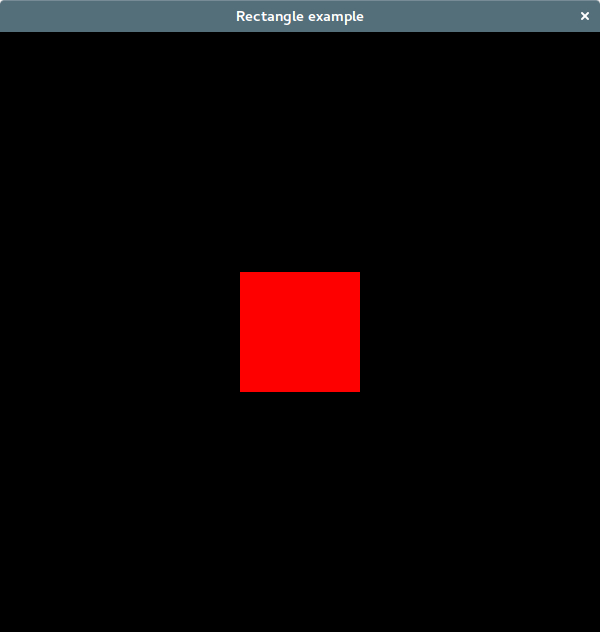
\includegraphics[width=0.7\textwidth]{rectangle_example}
    \caption{Rectangle example}
    \label{fig:rectangle_example}
\end{figure}

\subsection{Sprite}
A textured rectangle-shaped 1x1 Drawable

For different sizes use the scale in either the hum::Actor hum::Transform of
the Drawable's hum::Transform.

The following program draws a 20 by 20 cat image centered in a 100 by 100 area (camera 
defaults) scaled to 600 by 600.
\begin{lstlisting}[caption=Rectangle example]
#include "hummingbird/hum.hpp"
#include "MOGL/MOGL.hpp"

int main(void)
{
    hum::Game game;
    auto mogl = game.addPlugin<mogl::MultimediaOGL>(sf::VideoMode(600, 600), "Rectangle example");

    // load the texture and let the manager handle its lifetime
    mogl->textures().load("cat", "cat.jpg");

    auto actor = game.makeActor();
    actor->addBehavior<mogl::Sprite>(mogl->textures().get("cat"));
    actor->transform().position.x = 40;
    actor->transform().position.y = 40;
    actor->transform().scale.x = 20;
    actor->transform().scale.y = 20;

    game.run();
    return 0;
}
\end{lstlisting}

The result is the following capture:

\begin{figure}[H]
    \centering
    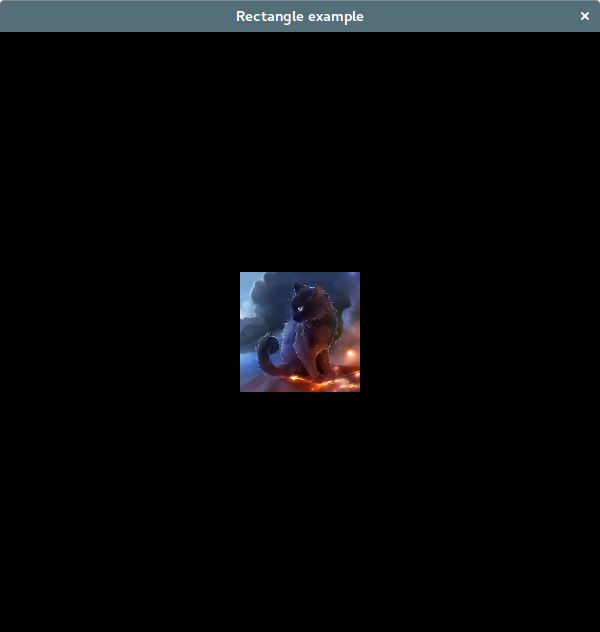
\includegraphics[width=0.7\textwidth]{sprite_example}
    \caption{Sprite example}
    \label{fig:sprite_example}
\end{figure}

\subsection{AnimatedSprite}
A textured rectangle-shaped 1x1 Drawable that changes over time.

For different sizes use the scale in either the hum::Actor hum::Transform of
the Drawable's hum::Transform.

The AnimatedSprite plays the animation defined in the SpriteAnimation assigned to it.

For an example of usage of both AnimatedSprite and SpriteAnimation see the section 
of the SpriteAnimationManager\ref{lst:spriteAnimationManager}

\subsubsection{SpriteAnimation}

A SpriteAnimation models an animation built from a sequence of frames stored in a 
tilesheet.

Given the following tilesheet:
\begin{figure}[H]
    \centering
    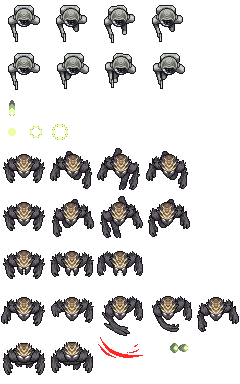
\includegraphics[width=0.7\textwidth]{sprites}
    \caption{sprites.png}
    \label{fig:sprites}
\end{figure}

The SpriteAnimation that stores the walking animation of the astronaut is defined 
in the next code fragment.

\begin{lstlisting}[caption=Astronaut walking animation]
mogl::SpriteAnimation walk{
  // texture containing the tilesheet
  game().getPlugin<mogl::MultimediaOGL>()->textures().get("sprites"),

  0,  // Horizontal offset of the tilesheet
  0,  // Vertical offset of the tilesheet
  0,  // Horizontal margin between tiles in the tilesheet
  0,  // Vertical margin between tiles in the tilesheet
  48, // Width of a tile in the tilesheet
  48, // Height of a tile in the tilesheet

  // Sequence of ids of the tiles in the tilesheet to play.
  {0, 1, 2, 3, 5, 6, 7, 8},

  // Sequence of hum::Times for each frame in the animation.
  std::vector(8, hum::Time::milliseconds(75))
};
\end{lstlisting}

\subsection{InputHandler}
Class that handles SFML input events and allows for easy quering of
related data.

Usage example:
\begin{lstlisting}[caption=InputHandler example]
mogl::InputHandler& input = game.getPlugin<mogl::MultimediaOGL>()->input();

// querying the keyboard
if (input.isKeyPressed(sf::Keyboard::Space))
{
    hum::log("Space has been pressed");
}

// querying the mouse
hum::Vector2i mouseDelta(0);
if (input.mouseMoved())
{
    mouseDelta = input.getMouseCurrentPosition() - input.getMousePreviousPosition();
}
\end{lstlisting}

\subsection{ResourceManagers}

\subsubsection{TextureManager}

A hum::ResourceManager for sf::Texture.

Example:
\begin{lstlisting}[caption=TextureManager example]
mogl::TextureManager tm;
tm.load("cat", "path/to/cat.jpg");
sf::Texture* cat = tm.get("cat");

//...

actor.addBehavior<mogl::Sprite>(cat);

//...

tm.free("cat");
\end{lstlisting}

\subsubsection{SpriteAnimationManager}

A hum::ResourceManager for mogl::SpriteAnimations.

This Resource manager is different because it uses SpriteAnimations as the
data to "load" and stores a copy of the given SpriteAnimation.

Example:
\begin{lstlisting}[caption=SpriteAnimationManager example, label=lst:spriteAnimationManager]
mogl::SpriteAnimation jump{
  // texture containing the tilesheet
  game().getPlugin<mogl::MultimediaOGL>()->textures().get("player"),
  0,  // Horizontal offset of the tilesheet
  0,  // Vertical offset of the tilesheet
  0,  // Horizontal margin between tiles in the tilesheet
  0,  // Vertical margin between tiles in the tilesheet
  48, // Width of a tile in the tilesheet
  48, // Height of a tile in the tilesheet
  {5, 6, 7, 8}, // Sequence of ids of the tiles in the tilesheet to play.
  std::vector(4, hum::Time::seconds(0.3f)) // Sequence of hum::Times for each frame in the animation.
};

mogl::SpriteAnimationManager sam;
sam.load("player_jump", jump);

//...

actor.addBehavior<mogl::AnimatedSprite>(sam.get("player_jump"));

//...

sam.free("player_jump");
\end{lstlisting}

\subsubsection{SoundManager}

A hum::ResourceManager for sf::SoundBuffers.

This Resource manager is different because it overwrites the get() method and
has other extra methods.

The SoundManager not just loads sf::SoundBuffers but also allows to play them
through the method play(). This method returns a std::pair containing the
id of the sound resource used (the one that is playing the required
sf::SoundBuffer) and a pointer to the sf::Sound managing the playback of the
sf::SoundBuffer. Note that a \textit{sound resource} is not the same as a sf::SoundBuffer.

The get() methods are also different. In this manager they are accessed by
sound ids (which are returned by play) and they return a pointer of the given
sf::Sound, or nullptr if the sound has been freed.

Example:
\begin{lstlisting}[caption= SoundManager example]
mogl::SoundManager sm;
sm.load("roar", "path/to/roar.ogg");

//...


// fixedUpdate()
if (event)
{
  roar_id = sm.play("roar", 50).first; // start playing the "roar" sound
}
// onDestroy()
if (sm.get(roar_id) != nullptr) // if the sound is still playing
{
  sm.get(roar_id)->stop(); // stop it
}

//...

sm.free("roar");
\end{lstlisting}

As shown in the example, when a sf::SoundBuffer playback is done (Stopped),
then the \textit{sound resource} is cleared and therefore the sound id invalidated
(getting its related sound returns nullptr).

Sound ids start at 1 and always grow, that means that a sound id of 0 will
always return nullptr.

\subsubsection{MusicManager}

A hum::ResourceManager for sf::Music.

Example:
\begin{lstlisting}[caption=MusicManager example]
mogl::MusicManager mm;
mm.load("music1", "path/to/music1.ogg");
sf::Music* music = mm.get("music1");
music->play();
//...
music->stop();
mm.free("music1");
\end{lstlisting}

\subsubsection{ShaderProgramManager}
A hum::ResourceManager for mogl::ShaderProgram.

This Resource manager is different because it uses ShaderProgramDefs to load
the resource (ShaderProgram) instead of the usual `std::string`.

Example:
\begin{lstlisting}[caption=ShaderProgramManager example]
// Create shaders
mogl::Shader vs, fs;

// Load vertex shader from file
vs.loadFromFile(Shader::Type::VERTEX_SHADER, "shader.vert");
if(!vs.isCompiled())
{
  hum::log_e("Vertex shader failed to compile: ", vs.log());
  return 1;
}

// Load fragment shader from file
fs.loadFromFile(Shader::Type::FRAGMENT_SHADER, "shader.frag");
if(!fs.isCompiled())
{
  hum::log_e("Fragment shader failed to compile: ", fs.log());
  return 1;
}

mogl::ShaderProgramDef def{vs, fs, "out_color"};

mogl::ShaderProgramManager spm;
spm.load("plain_shader", def);

mogl::ShaderProgram* sp = spm.get("plain_shader");
sp->use()->setUniform4f("color", 0, 1, 1, 1);

// ...

spm.free("plain_shader");
\end{lstlisting}



\chapter{Game implementation example}

TODO

\section{Player}

This class implements the Behavior for the Player (the astronaut). It implements 
the movement, using the keyboard, and displays it on screen. The player has a health 
bar on top of it. The main problem is that we'll be rotating the player actor and thus, 
any Drawable attached to it will also rotate, therefore what we'll do to display the health 
bar is to have another actor that mimics all movement of the player, except for the rotation. 
We'll call this actor the helper.

Below the class code is exposed and explained.

\begin{lstlisting}
#ifndef PLAYER_HPP
#define PLAYER_HPP
#include "hummingbird/hum.hpp"
#include "MOGL/MOGL.hpp"
#include "Bullet.hpp"
#include "Resources.hpp"
#include "math.hpp"

class Player : public hum::Behavior
{
private:
    static int s_lives;
    static float s_vel;
    static unsigned int s_ms_shoot;

    int p_live;
    mogl::MultimediaOGL* p_mogl;
    mogl::AnimatedSprite* p_sprite;
    hum::Kinematic* p_kinematic;
    hum::Kinematic* p_helper_kinematic;
    mogl::Rectangle* p_live_rectangle;
    float p_prev_rotation;
    hum::Clock p_clock;

\end{lstlisting}

We start by including the required files. First, we include Hummingbird and MOGL. 
Then, the various files for the game that are used by the player: Bullet.hpp (the projectile 
shot by the player), Resources.hpp (includes some functions for loading configuration files) and 
math.hpp (includes \texttt{cmath} and implements the method \texttt{square(float x)}, useful for 
calculating distances). We'll see those files in more detail later.

Next, we define the Player class, which is a Behavior, and its private methods.  The 
static variables are used for storing class wise configuration values, read from a 
configuration file on the first instantiation of the class. Then we store useful information, 
such as the number of lives that the player has left and pointers to useful components 
such as the kinematic behavior of the player actor and the helper actor; MOGL, for 
accessing input information; the sprite of the player and the rectangle of the health 
bar; and a clock for measuring time, such as the time between shots.

\begin{lstlisting}
public:
    Player()
    {
        if (s_vel == -1)
        {
            std::stringstream ss;
            readFileContents("res/config/Player.cfg", ss);
            ss
                >> s_vel
                >> s_ms_shoot
                >> s_lives;
        }
    }
\end{lstlisting}

As commented before, the first time a Player is instantiated the configuration is read 
from a file. This avoids having to recomplile the project for adjusting gameplay values.

Afterwards, the initialitazion function of the Behavior is defined. We use it to 
give the player actor all behaviors and configuration needed, such as adding the 
AnimatedSprite to it and creating the helper actor for the health bar.

\begin{lstlisting}
    void init() override
    {
        // get the MOGL plugin instance and store it
        p_mogl = actor().game().getPlugin<mogl::MultimediaOGL>();

        // get the SpriteAnimation, that has already been loaded before
        // game start, and create the AnimatedSprite with it.
        mogl::SpriteAnimation* player_animation =
            p_mogl->spriteAnimations().get("player");
        p_sprite =
            actor().addBehavior<mogl::AnimatedSprite>(player_animation);
        // Set the animation to pause as the player is not moving.
        p_sprite->pause();
        // fix the rotation of the sprite.
        p_sprite->transform().rotation.z = -90;

        // Set the center for transformations of the sprite to the center
        // of the astronaut tile (a bit displaced from the actual center
        // of the 48 by 48 tile)
        p_sprite->setOrigin(hum::Vector3f(24./48., 18./48., 0));

        // Add kinematic behavior to the player actor and store a pointer
        // to it
        p_kinematic = actor().addBehavior<hum::Kinematic>();

        // set other useful information
        p_prev_rotation = 0;
        p_live = s_lives;

        // Create the helper actor we don't need to save a pointer to it,
        // as we will mainly work with its Kinematic Behavior and said
        // behavior has a reference to its actor.
        hum::Actor* helper = actor().game().makeActor();
        // Sync the transformations
        helper->transform() = actor().transform();
        // Add Kinematic, save it and sync it with the player's one.
        p_helper_kinematic = helper->addBehavior<hum::Kinematic>();
        helper->transform().position.z = -0.5;
        helper->transform().position.y -= 0.8;
        helper->transform().position.x -= 0.4;

        // Add the background of the health bar
        auto rect =
            helper->addBehavior<mogl::Rectangle>(sf::Color::White);
        rect->transform().scale = hum::Vector3f(0.8, 0.1, 0.02);

        // Add the foreground color of the health bar (the actual
        // indicator)
        p_live_rectangle =
            helper->addBehavior<mogl::Rectangle>(sf::Color::Green);
        p_live_rectangle->transform().scale =
            hum::Vector3f(0.8, 0.1, 0.02);
        p_live_rectangle->transform().position.z = -0.1;
    }
\end{lstlisting}

Now we need to implement the update method of the player. We will read the input using 
the InputHandler instance inside the MOGL plugin and update the player's speed depending 
on it. We'll also create Bullets if the user presses the left mouse button.

\begin{lstlisting}
    void fixedUpdate() override
    {
        if (isDead())
        {
            p_sprite->stop();
            p_kinematic->velocity().position.x = 0;
            p_kinematic->velocity().position.y = 0;
            p_kinematic->velocity().rotation.z = 0;

            p_helper_kinematic->velocity().position.x =
                p_kinematic->velocity().position.x;
            p_helper_kinematic->velocity().position.y =
                p_kinematic->velocity().position.y;
            return;
        }
\end{lstlisting}

First thing, if the player is dead, do nothing. Otherwise, update the rotation and movement 
speed.

\begin{lstlisting}
        // Look at the mouse
        hum::Vector2f mouse = p_mogl->input().getMouseCurrentPosition();
        mouse /= 48.f;
        float x = mouse.x - actor().transform().position.x;
        float y = mouse.y - actor().transform().position.y;
        float angleInRadians = std::atan2(y, x);
        float angleInDegrees = (angleInRadians / M_PI) * 180.0;
        float delta = angleInDegrees - p_prev_rotation;
        if (delta > 180)
        {
            delta -= 360;
        }
        else if (delta < -180)
        {
            delta += 360;
        }
        p_kinematic->velocity().rotation.z =
            delta / actor().game().fixedUpdateTime().asSeconds();
        p_prev_rotation = angleInDegrees;
\end{lstlisting}

In the fragment above, we first get the current position of the mouse and we transform 
it to game world coordinates by dividing it by 48. This is because in the main funtion 
we set the window to be 1000 by 1000 pixels, but the viewport to display 1 by 1 squares 
as 48 by 48 pixels on screen.  We do this because, by default, all Drawables are 1 
by 1 of size in the game world. To avoid having to set scales to all of them, we scale 
the view.

Then, we calcultate the angle from the player's position to the mouse position and, from it, 
the speed at which the player is rotating. This is where \texttt{p\_prev\_rotation} becomes useful.

\begin{lstlisting}
        // Movement
        if (p_mogl->input().isKeyDown(sf::Keyboard::A))
        {
            p_kinematic->velocity().position.x =
                -s_vel * (not p_mogl->input().isKeyDown(sf::Keyboard::D));
        }
        else if (p_mogl->input().isKeyDown(sf::Keyboard::D))
        {
            p_kinematic->velocity().position.x = s_vel;
        }
        else
        {
            p_kinematic->velocity().position.x = 0;
        }

        if (p_mogl->input().isKeyDown(sf::Keyboard::W))
        {
            p_kinematic->velocity().position.y =
                -s_vel * (not p_mogl->input().isKeyDown(sf::Keyboard::S));
        }
        else if (p_mogl->input().isKeyDown(sf::Keyboard::S))
        {
            p_kinematic->velocity().position.y = s_vel;
        }
        else
        {
            p_kinematic->velocity().position.y = 0;
        }

        if (p_kinematic->velocity().position.x != 0
            or p_kinematic->velocity().position.y != 0)
        {
            p_sprite->play();
        }
        else
        {
            p_sprite->pause();
        }
\end{lstlisting}

For the movement, we just query the keyboard for the status of the direction keys: 
\textbf{A}, \textbf{S}, \textbf{D}, \textbf{W}.  And depending on the input, set the 
speed of the actor. Finally, if the player is moving, play the animation; pause it 
otherwise.

For shooting we check if the mouse left button is pressed and if the minimum time between shots 
has passed. The time is checked by using the clock.

\begin{lstlisting}
        // Shooting
        if (p_mogl->input().isMouseButtonDown(sf::Mouse::Left)
            and p_clock.getTime().asMilliseconds() >= s_ms_shoot)
        {
            auto bullet = actor().game().makeActor();
            float mod = sqrt(square(x) + square(y));
            x /= mod;
            y /= mod;
            bullet->addBehavior<Bullet>(x, y);
            bullet->transform().position.x =
                actor().transform().position.x + 0.6 * x - 0.14 * y;
            bullet->transform().position.y =
                actor().transform().position.y + 0.6 * y + 0.14 * x;
            p_clock.reset();
        }
\end{lstlisting}

If the conditions for shooting are met, we create a new actor, add to it a Bullet Behavior, 
give a direction to it and place it infront of the player. Lastly, we reset the clock.

\begin{lstlisting}
        p_helper_kinematic->velocity().position.x =
            p_kinematic->velocity().position.x;
        p_helper_kinematic->velocity().position.y =
            p_kinematic->velocity().position.y;

        sf::Listener::setPosition(
            actor().transform().position.x,
            actor().transform().position.y,
            10);
    }
\end{lstlisting}

At the end of the update we sync the helper kinematic and set the position of the listener (sounds).

\begin{lstlisting}
    void hit()
    {
        if (not isDead())
        {
            --p_live;
            p_live_rectangle->transform().scale.x =
                (float)p_live/s_lives * 0.8;
        }
    }

    bool isDead() const
    {
        return (p_live <= 0);
    }
};
float Player::s_vel = -1;
unsigned int Player::s_ms_shoot;
int Player::s_lives;
#endif
\end{lstlisting}

Finally, we implement some functions allowing other classes to interact with the player and 
we initialize the static members.

\section{Enemy}

This class implements the Behavior for the Enemy of the game. its AI is defined as 
state machine, represented in figure \ref{fig:enemy_AI}, and thus the update method is divided in the various states it can be. 

\begin{figure}[h]
    \centering
    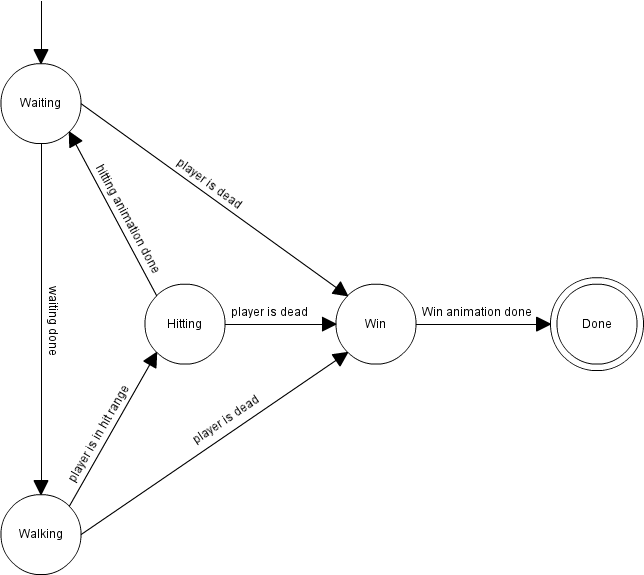
\includegraphics[width=0.8\textwidth]{enemy_AI}
    \caption{Flow chart of the Enemy's AI}
    \label{fig:enemy_AI}
\end{figure}

\begin{lstlisting}
#ifndef ENEMY_HPP
#define ENEMY_HPP
#include "hummingbird/hum.hpp"
#include "MOGL/MOGL.hpp"
#include "Resources.hpp"
#include "Player.hpp"
#include "math.hpp"

class Enemy : public hum::Behavior
{
private:
    enum State { WALKING, HITTING, WAITING, WIN, DONE };

    static float s_vel;
    static float s_min_player_dist;

    hum::Clock p_clock;
    State p_status;
    Player* p_player;
    hum::Kinematic* p_kinematic;
    float p_prev_rotation;
    mogl::AnimatedSprite* p_sprite;
    mogl::AnimatedSprite* p_blood;
    mogl::MultimediaOGL* p_mogl;
    mogl::SoundId p_sound;

public:
    // Enemy's AI states
    enum State { WALKING, HITTING, WAITING, WIN, DONE };

    Enemy(Player* player):
    p_player(player),
    p_sound(0)
    {
        if (s_vel == -1)
        {
            std::stringstream ss;
            readFileContents("res/config/Enemy.cfg", ss);
            ss >> s_vel;
            ss >> s_min_player_dist;
        }
    }
\end{lstlisting}

As in the Player class, we include the required files, define private variables to 
store useful information and use the constructor for reading the class configuration. Some 
of the private information is similar to the player's one.

Enemy receives a pointer to the player in its constructor, we store it. We'll use it 
to check if the player is in hitting range and if so hit it.

Unlike Player, Enemy has two AnimatedSprites. The first is the one that plays the various 
enemy animations: walking, hitting, winning; the second plays the blood animation, only 
show when the player is hit. Finally, the we store a SoundId to handle the playback of 
the various sounds the Enemy can produce: hit and roar.

\begin{lstlisting}
    void init() override
    {
        p_kinematic = actor().addBehavior<hum::Kinematic>();
        p_prev_rotation = 0;

        p_mogl = actor().game().getPlugin<mogl::MultimediaOGL>();
        p_sprite = actor().addBehavior<mogl::AnimatedSprite>(p_mogl->spriteAnimations().get("enemy_walking"));
        p_sprite->pause();
        p_sprite->setOrigin(hum::Vector3f(24./48., 18./48., 0));
        actor().transform().rotation.z = -90;

        p_blood = actor().addBehavior<mogl::AnimatedSprite>(p_mogl->spriteAnimations().get("enemy_attack1_blood"));
        p_blood->setLooping(false);
        p_blood->stop();
        p_blood->disable();
        p_blood->setOrigin(hum::Vector3f(24./48., -10./24., 0));

        p_status = WAITING;
    }
\end{lstlisting}

Like in Player, we use the initialitazion method for configuring the actor. We add 
the Kinematic Behavior and the AnimatedSprites, setting each of them accordingly. Finally, 
we set the initial AI state.

Enemy also needs to handle its destruction, as it uses sound resources. We release them, 
by stoping the sound we indicate it is done and MOGL will take care of freeing it.

\begin{lstlisting}
    void onDestroy() override
    {
        if (p_mogl->sounds().get(p_sound) != nullptr)
        {
            p_mogl->sounds().get(p_sound)->stop();
        }
    }
\end{lstlisting}

Now it is when the fun comes: the update. The first thing we do is to define the \textit{base} 
state changes: if the Enemy is \textbf{done}, do nothing; and if the player dies, 
change to \textbf{win} state.

In the \textbf{win} state, the Enemy does nothing, just waits one second still. Therefore, we 
stop all animations and reset the clock to mesure the second.

\begin{lstlisting}
    void fixedUpdate() override
    {
        if (p_status == DONE)
        {
            return;
        }

        if (p_player->isDead() and p_status != DONE and p_status != WIN)
        {
            p_status = WIN;
            p_sprite->stop();
            p_blood->disable();
            p_clock.reset();
        }
\end{lstlisting}

Next, we calculate the rotation speed of the Enemy. This step is the same as the player, 
with the difference that the position to look at is not the mouse but the player. We 
also calculate the distance between the enemy and the player and set the speed of the 
enemy to 0.

\begin{lstlisting}

        // Look at the player
        float x = p_player->actor().transform().position.x - actor().transform().position.x;
        float y = p_player->actor().transform().position.y - actor().transform().position.y;
        float angleInRadians = std::atan2(y, x);
        float angleInDegrees = (angleInRadians / M_PI) * 180.0;
        float delta = angleInDegrees - p_prev_rotation;
        if (delta > 180)
        {
            delta -= 360;
        }
        else if (delta < -180)
        {
            delta += 360;
        }
        p_kinematic->velocity().rotation.z = delta / actor().game().fixedUpdateTime().asSeconds();
        p_prev_rotation = angleInDegrees;

        p_kinematic->velocity().position.x = 0;
        p_kinematic->velocity().position.y = 0;

        // distance between the enemy and the player
        float mod = sqrt(square(x) + square(y));
\end{lstlisting}

If the enemy is in \textbf{win} state and the one second still time has passed, the 
enemy changes to \textbf{done} state and starts the win animation. We set the animation 
not to loop so that it stops when done.

\begin{lstlisting}
        if (p_status == WIN)
        {
            if (p_clock.getTime().asSeconds() > 1)
            {
                p_sprite->setSpriteAnimation(p_mogl->spriteAnimations().get("enemy_win"));
                p_sprite->setLooping(false);
                p_sprite->play();
                p_status = DONE;
            }
        }
\end{lstlisting}

On the other hand, if the enemy is \textbf{walking} and the player is not in hitting range 
the enemy moves towards the player. We set the speed, play the walking animation if 
not playing already and, with a probability of 0.01, play the \textit{roar} sound if 
no sound is playing. We store the SoundId of the roar sound so that we know if the 
enemy is still roaring or not.

\begin{lstlisting}
        else if (p_status == WALKING and s_min_player_dist < mod)
        {
            x /= mod;
            y /= mod;
            p_kinematic->velocity().position.x = x * s_vel;
            p_kinematic->velocity().position.y = y * s_vel;
            if (p_sprite->status() != mogl::AnimatedSprite::Status::PLAYING)
            {
                p_sprite->play();
            }

            if (p_mogl->sounds().get(p_sound) == nullptr and (rand()%100) > 99)
            {
                auto info = p_mogl->sounds().play("roar", 1000);
                info.second->setAttenuation(0.1);
                p_sound = info.first;
            }
        }
        else
        {
            if (p_status != WAITING)
            {
                if (p_status != HITTING) // state == WALKING and player is in hitting distance
                {
\end{lstlisting}

If the enemy is \textbf{walking} and the player is in hitting distance, the enemy changes 
to \textit{hitting} state. Changes the animation of the sprite and sets it not to loop, 
this way we can check when the animation is done and change to the next state. Finally, 
we play the sound of the enemy's attack and set its position and attenuation. In this case, 
we don't need to store the SoundId because we know that the hit sound will finish before the 
enemy is able to hit again.

\begin{lstlisting}
                    p_sprite->setSpriteAnimation(p_mogl->spriteAnimations().get("enemy_attack1"));
                    p_sprite->play();
                    p_sprite->setLooping(false);
                    p_status = HITTING;
                    sf::Sound* sound = p_mogl->sounds().play("enemy_attack", 50).second;
                    sound->setPosition(actor().transform().position.x, actor().transform().position.y, 0);
                    sound->setAttenuation(0.01);
                }
                else
                {
\end{lstlisting}

If the state is \textbf{hitting} and the hitting animation has finished, the status 
changes to \textbf{waiting}. We set the animation back to walking and disable the blood 
AnimatedSprite, in case it was displayed. The clock is also resetted so that we can mesure 
the waiting time.

\begin{lstlisting}
                    if (p_sprite->status() == mogl::AnimatedSprite::Status::STOPPED)
                    {
                        p_sprite->setSpriteAnimation(p_mogl->spriteAnimations().get("enemy_walking"));
                        p_sprite->setLooping(true);
                        p_status = WAITING;

                        p_blood->stop();
                        p_blood->disable();

                        p_clock.reset();
                    }
\end{lstlisting}

Else, if the hitting animation hasn't finished but it just passed the frame where the 
hit happens, check if the player is still in range and if so, hit it and display blood.

\begin{lstlisting}
                    else if (p_sprite->frameIndex() > 1 and not p_blood->isEnabled())
                    {
                        if (mod < s_min_player_dist)
                        {
                            p_blood->enable();
                            p_blood->play();
                            p_player->hit();
                        }
                    }
                }
            }
            else
            {
\end{lstlisting}

Finally, if the enemy is in \textbf{waiting} state, check if the waiting time has 
passed and if so, set the state to \textbf{walking}.

\begin{lstlisting}
                hum::Time t = p_clock.getTime();
                if (t.asSeconds() > 1)
                {
                    p_status = WALKING;
                }
            }
        }
\end{lstlisting}

As a last detail, if the \textit{roar} sound is being played, update its position.
\begin{lstlisting}
        sf::Sound* sound = p_mogl->sounds().get(p_sound);
        if (sound != nullptr)
        {
            sound->setPosition(actor().transform().position.x, actor().transform().position.y, 0);
        }
    }

    static const char* behaviorName()
    {
        return "Enemy";
    }
};
float Enemy::s_vel = -1;
float Enemy::s_min_player_dist = -1;
#endif
\end{lstlisting}

\section{Bullet}

This class implenst the behavior of a bullet shot by the player. The bullet has a lifespan of 
half a second and if while alive it hits an Enemy it kills it and destroys itself.

\begin{lstlisting}
#ifndef BULLET_HPP
#define BULLET_HPP
#include "hummingbird/hum.hpp"
#include "MOGL/MOGL.hpp"
#include "Resources.hpp"
#include "math.hpp"

class Enemy;
class Bullet : public hum::Behavior
{
private:
    static float s_vel;
    float p_comp_x, p_comp_y;
    hum::Clock clk;
    hum::Kinematic* p_kinematic;
    mogl::Sprite* p_bullet;
    mogl::AnimatedSprite* p_explode;

public:
    Bullet(float comp_x, float comp_y):
    p_comp_x(comp_x),
    p_comp_y(comp_y)
    {
        if (s_vel == -1)
        {
            std::stringstream ss;
            readFileContents("res/config/Bullet.cfg", ss);
            ss >> s_vel;
        }
    }

    void init() override
    {
        mogl::MultimediaOGL* mogl = actor().game().getPlugin<mogl::MultimediaOGL>();

        p_explode = actor().addBehavior<mogl::AnimatedSprite>(mogl->spriteAnimations().get("bullet_explosion"));
        p_explode->disable();
        p_explode->setLooping(false);
        p_explode->setOrigin(hum::Vector3f(12./24., 12./24., 0));
        p_explode->transform().scale.x = 0.5;
        p_explode->transform().scale.y = 0.5;

        p_bullet = actor().addBehavior<mogl::Sprite>(mogl->textures().get("sprites"), sf::IntRect(0, 96, 24, 24));
        p_bullet->transform().scale.x = 0.5;
        p_bullet->transform().scale.y = 0.5;
        p_bullet->setOrigin(hum::Vector3f(12./24., 18./24., 0));

        float angleInRadians = std::atan2(p_comp_y, p_comp_x);
        float angleInDegrees = (angleInRadians / M_PI) * 180.0;
        p_bullet->transform().rotation.z = angleInDegrees - 90;

        p_kinematic = actor().addBehavior<hum::Kinematic>();
        p_kinematic->velocity().position.x = p_comp_x * s_vel;
        p_kinematic->velocity().position.y = p_comp_y * s_vel;

        mogl->sounds().play("gun_shot", 40, false, true);
        clk.reset();
    }
\end{lstlisting}

The Bullet stores its direction, Kinematic, the Sprite for displaying the actual bullet and 
an AnimatedSprite for playing the explosion when being destroyed.

As in previous Behaviors, we use the constructor to read the configuration only once and 
we also store the direction oin which the bullt will move.

Then, on initialization, we again add the required Behaviors to the actor and set their values 
to properly display and move the bullet. First, we add the animation for the explosion of 
the bullet, we disable it so that it doesn't display anything and we center it to the actor's 
position. Next, we add the actual bullet sprite and, again, we center it and rotate it 
towards the movement's direction. Following that, we add the Kinematic and set the speed and, finally, 
we play the \textit{gun\_shot} sound and reset the clock to measure the bullet's lifetime.

\begin{lstlisting}
    void fixedUpdate() override
    {
        if (clk.getTime().asSeconds() > 0.5 and not p_explode->isEnabled())
        {
            p_bullet->disable();
            p_explode->enable();
            p_kinematic->velocity().position.x = 0;
            p_kinematic->velocity().position.y = 0;
        }
        else if (p_explode->status() == mogl::AnimatedSprite::Status::STOPPED)
        {
            actor().game().destroy(actor());
        }
        else if (not p_explode->isEnabled())
        {
            // Get the set of actors in the game
            auto& actors = actor().game().actors();
            float x, y, mod;

            // For each actor...
            for (auto it = actors.begin(); it != actors.end(); ++it)
            {
                hum::Actor* a = *it;
                x = a->transform().position.x - actor().transform().position.x;
                y = a->transform().position.y - actor().transform().position.y;
                mod = sqrt(square(x) + square(y));
                // ... if it is near enough ...
                if (mod < 0.52)
                {
                    // ... and if it is an Enemy, ...
                    try
                    {
                        a->getBehavior<Enemy>();
                    }
                    catch (hum::exception::BehaviorNotFound e)
                    {
                        continue;
                    }
                    // ... kill it and destroy the bullet
                    actor().game().destroy(*a);
                    p_bullet->disable();
                    p_explode->enable();
                    p_kinematic->velocity().position.x = 0;
                    p_kinematic->velocity().position.y = 0;
                    break;
                }
            }
        }
    }
};
float Bullet::s_vel = -1;
#endif
\end{lstlisting}

The Bullet's fixed update is quite simple. First, it checks if the bullet has lived over 
its livespan and, if so, starts the explosion animation. Next, it checks if the explosion 
animation is over and destroys the bullet if so. Finally, it iterates through all the Actors in 
the game; checks if they are in hit range and if they are of type Enemy; and if they are enemies 
it kills the enemy and plays the explosion animation.


\chapter{Future work}\label{ch:future_work}

The Hummingbird framework and MOGL, although functional, are far from being complete. 
The following list is a sample of what could be done to improve and extend the project.

\begin{itemize}
\item \textbf{Data locality}: Proper object pools for Actors and Behaviors to take advantage of caching
and avoid the iteration over inactive Actors and Behaviors.
\item \textbf{Hide the glm dependencie from the user}: Use only glm classes internaly, to the point that 
the eventual user of the MOGL plugin doesn't need to know it is used inside (as in not having to include its headers).
\item \textbf{3D rendering}: implement more Drawable Behaviors for rendering arbitrary 3D geometry.
\end{itemize}

There is a lot that can be done, in the end this is just the core of what a game 
engine is and inside every part of a game engine lots of tweaking can be done.

\chapter{Project planning}\label{ch:project_planning}

\section{Methodology and rigor}

This project will be developed using the Agile\cite{agilemanifesto} method with sprints 
of one week. All tasks will be written as tickets in a Trello\cite{trello} board. 
The board will consist of five lists: Backlog, To Do, In Progress, Done, Archive. 
The workflow with this lists is explained bellow.

First, all tasks created are put in the Backlog list. Once a week, every beginning 
of sprint iteration, the progress on the tickets assigned for the ending iteration 
is reviewed and the tickets in Done are moved to Archive.

Next, new tickets from Backlog are moved to To Do, bearing in mind the tickets that 
are still in To Do and In Progress (if any). The tickets put in To Do are the goal 
for the starting sprint and, ideally, will be done before the next one.

During the sprint, when picking a new ticket from To Do, it is moved to In Progress 
to make it clear that this is being worked on. This makes it easier to keep track 
of the progress during the sprint. When a ticket in progress is done, it is moved 
from In Progress to Done.

I chose this system because it allows for fast iteration on the implementation and 
enables me to adapt to changes or unexpected obstacles I may find. It also gives me 
feedback on my progress on-live as it is represented in the Trello board.

The described process will be approached, from a development point of view, using 
Git for version management and the feature branching\cite{featurebranching} technique 
for each ticket. Merging each feature branch into master once the implementation has 
been tested to work properly.  This workflow allows to simultaneously work on multiple 
tickets having each of them encapsulated in their respective branches and ensures 
that master branch never contains broken code.

Finally, to validate that the goals of this project have been achieved it's only needed 
to refer to the scope exposed previously in this document and go through the list 
of features that must be implemented.

\section{Description of tasks}

In this section I'll list and explain the tasks required to fulfill the project's 
objective. These tasks are sorted by requirements, that is, every task requires the 
one before it to be able to start working on it. For all of the tasks a Laptop PC 
will be needed.

\subsection{Project planning}

This task consist mainly in all the tasks that the GEP course covers. It contains 
the following subtasks:

\begin{itemize}
\item Context and scope definition
\item Temporal planning
\item Budget and sustainability
\end{itemize}

This first task is very important, as it lays out the path for the whole project. 
It makes everything else almost straightforward as the overall view of the project 
is already thought.

The dependencies between the tasks are defined by the order they are presented. That 
means that the task 2 requires the task 1 to be done before being able to work on 
it, and so on with the following tasks.

\subsection{Game framework}

This is the main task for the project. It consist on the development, testing and 
documentation of all the parts that conform the game framework. This main task can 
be divided in the subtasks explained in the following sections.

\subsubsection{Helper classes}

This task consists of developing a set of classes containing general functionality 
for game development. These functionalities consist of describing spatial transformation 
of objects, measuring time and storing intervals of time. These functionalities will 
be encapsulated in the following classes, respectively: \textit{Transformation},
\textit{Clock}, \textit{Time}.

\subsubsection{Actor and Behavior classes}

This task consists of designing the behavior system and implementing the \textit{Behavior} 
virtual class. It also includes implementing the \textit{Actor} class, which will 
mainly be a container for behaviors, and its interface for being able to update the 
game state.


\subsubsection{Game class}

The \textit{Game} class implements the main loop and contains the actor pool. At this stage 
this class won't include the plug-in system, that will be implemented afterwards. 
Moreover, this task will also include extensive testing of all the system up to this 
point, looking for bugs and memory leaks.

\subsubsection{Plug-in system}

After the \textit{Game} class is implemented and thoroughly tested, comes this task. 
It consists in adding the plug-in system to the \textit{Game} class. That is, designing 
and implementing the \textit{Plugin} virtual class and extending the \textit{Game} 
class to handle the plug-ins.

Once this task is done, the framework is completed and ready to use.

\subsection{SFML plug-in (MOGL)}

This task consists in developing a \textit{Plugin} for the game framework that wraps 
the SFML functionality in a way that is useful for developing 2D games with the framework 
and this plug-in.

\subsubsection{Resource Managers}

All games have resources that occupy space in memory such as textures or sounds among 
others. This task consists in developing managers for these resources to handle them 
efficiently.

\subsubsection{Input handler}

User input is what makes a game really a game, otherwise it'd be some kind of movie. 
This task will focus on implementing a data structure that stores the state of the 
input and allows querying that state in a simple way.


\subsubsection{Drawable classes}

This task consists on designing a \textit{Drawable} interface for \textit{Behavior}s 
that have a drawable representation. Then, implement the following drawable behaviors:

\begin{itemize}
\item \textit{Rectangle}, a plain colored rectangle;
\item \textit{Circle}, a plain colored circle;
\item \textit{ConvexShape}, a plain colored convex polygon;
\item \textit{Text}, text using a font;
\item \textit{Sprite}, a static image from a texture;
\item \textit{AnimatedSprite}, a animation from a series of images in a given texture (tile 
sheet).
\end{itemize}

All drawable behaviors will have their own transformation, relative to their actor.

\subsubsection{MultimediaOGL class}

The \textit{MultimediaOGL} class will contain the logic for the rendering pipeline 
of the drawable behaviors, the input handles and the resource managers.

Again, at this point all the previous work will be extensively tested to find possible 
bugs and memory leaks.

\subsection{Final task}

This task is about making sure that all the documentation is done, reviewed to prepare 
the final presentation.

\section{Time table}

The following table summarizes the time that will be spent for each of the tasks described 
previously.

\begin{figure}[h]
    \centering
    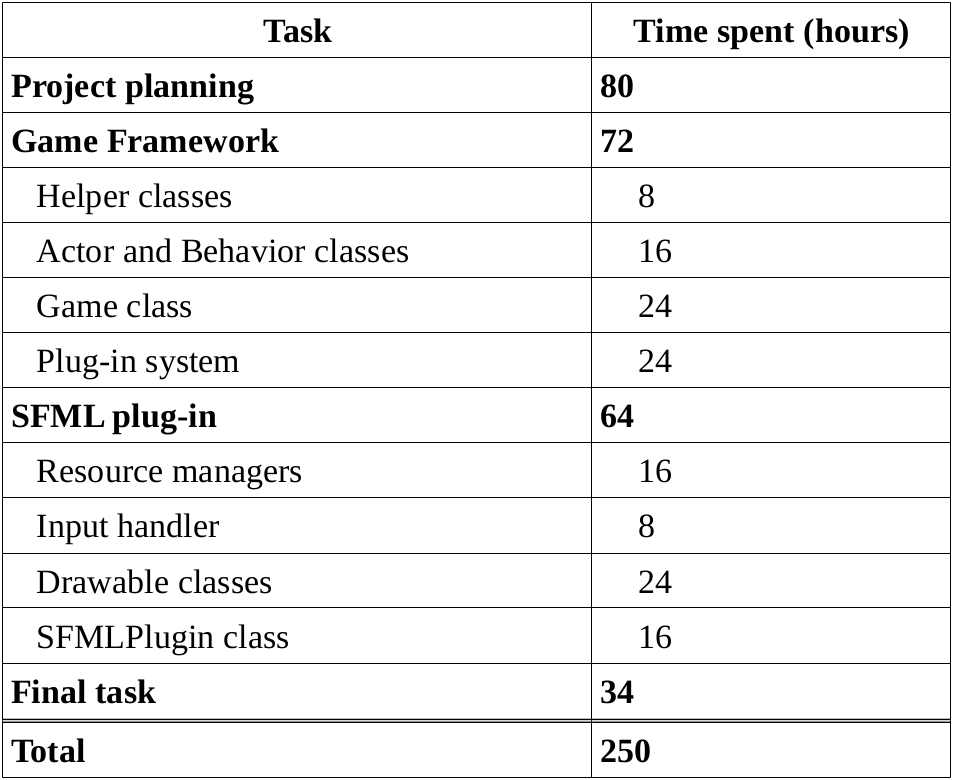
\includegraphics[width=0.8\textwidth]{time_table}
    \caption{Time spent per task}
    \label{fig:time_table}
\end{figure}


\section{Gantt chart}

The planned schedule is represented in the following Gantt chart. I've considered 
a working day of 4 hours a day for this schedule, as this will be approximately the 
time available to dedicate to the project.

\begin{figure}[H]
    \centering
    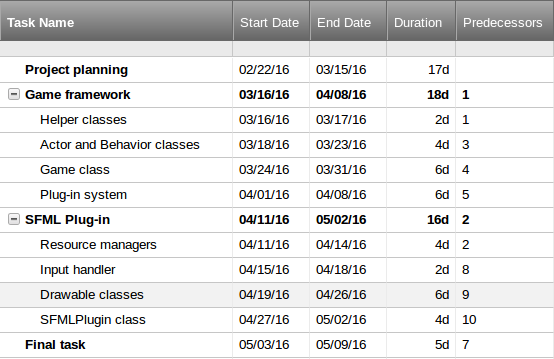
\includegraphics[width=0.8\textwidth]{tasklist}
    \caption{Time planning of tasks}
    \label{fig:time_planning}
\end{figure}
\begin{figure}[H]
    \centering
    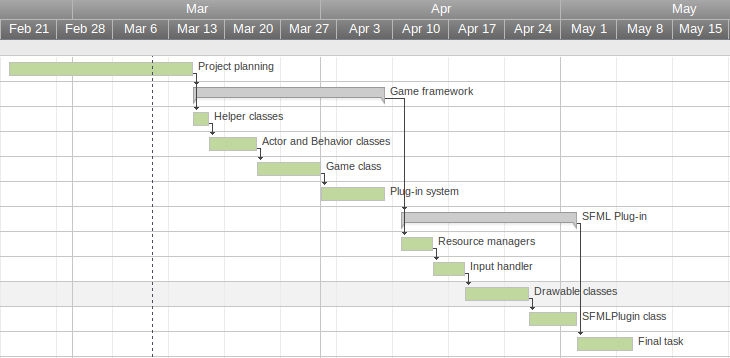
\includegraphics[width=\textwidth]{gantt_chart}
    \caption{Gantt chart of the project}
    \label{fig:gantt_chart}
\end{figure}


\section{Action plan}

The idea is to follow the plan as described above, completing tasks in the specified 
order and inside their planned time span.
The plan described in the Gantt chart consists of a schedule of 4 hours a day and 
does not include weekends. If at some point there is some kind of obstacle that may 
slow the development of one of the tasks it is possible to work on weekends to get 
up-to-date with the planning.

Each task that consists of development also includes the documentation of said piece 
of code using Doxygen. This way, when the implementation is done I'll immediately 
have its documentation without having to go back into the code.

Every time a major task is completed a meeting with the project director is to be 
scheduled to review the progress.

In the case of an unexpected extraordinary delay, the project planning will be adjusted 
accordingly by taking advantage of the time available between the planned ending of 
the project and the presentation date.


\section{Budget estimation}

For this section I am going to present an estimation of the budget needed to make 
the project possible. The costs will be divided in three groups depending on their 
type. These types are software, hardware and human resources.

To calculate the amortization I'll consider the useful life of the resource and that 
the project will last 56 days, following the planning.

\subsection{Hardware resources}

The table below lists the hardware resources needed for the realization of the project, 
their cost and amortization.
\begin{figure}[H]
    \centering
    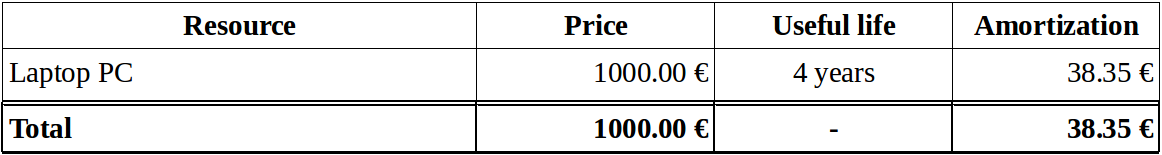
\includegraphics[width=\textwidth]{hardware_res}
    \caption{Hardware resources}
    \label{fig:hardware_res}
\end{figure}

\subsection{Software resources}

The next table lists the software resources needed for the project in the same format 
as the previous section.
\begin{figure}[H]
    \centering
    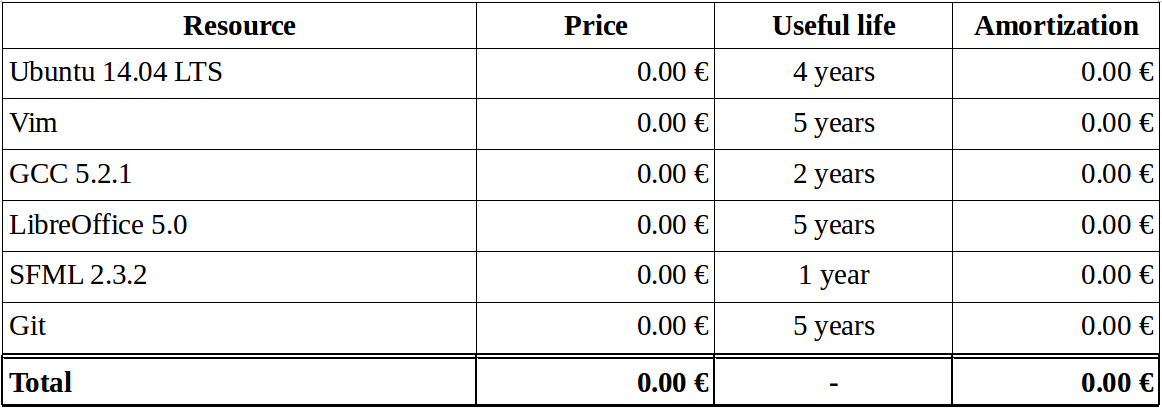
\includegraphics[width=\textwidth]{software_res}
    \caption{Software resources}
    \label{fig:software_res}
\end{figure}

\subsection{Human resources}

The table shows the costs for the human resources needed in the development of the 
project. The cost is calculated assuming a 4 hours per day schedule.
\begin{figure}[H]
    \centering
    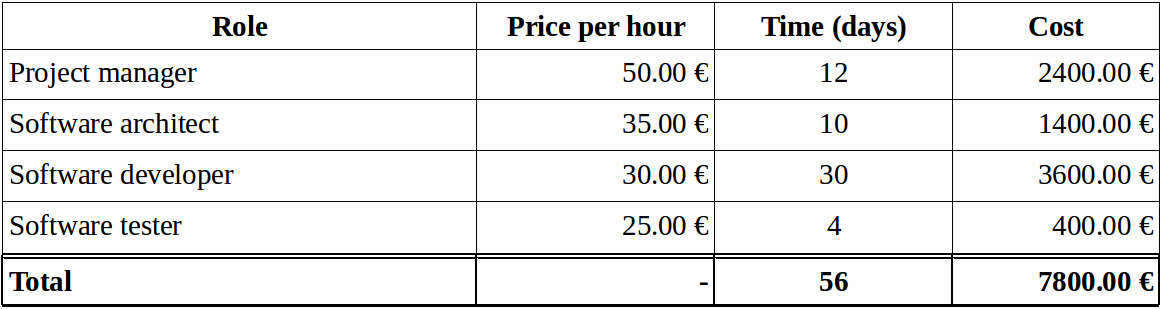
\includegraphics[width=\textwidth]{human_res}
    \caption{Human resources}
    \label{fig:human_res}
\end{figure}

Each of these different roles will be assigned different tasks in the project. Specifically, 
the \textit{Project manager} will be assigned to almost the whole \textit{Project 
planning} task and the \textit{Final task}; the \textit{Software architect} will work 
at the ending part of the \textit{Project planning} determining the blueprints for 
the development of the project; the \textit{Software developer} will take care of 
the whole development; and the \textit{Software tester} will test the project when 
new milestones are reached during the development task.

\subsection{Total budget}

From the estimations in previous sections the following summary can be obtained, showing 
the total budget for the development of the project.

\begin{figure}[h]
    \centering
    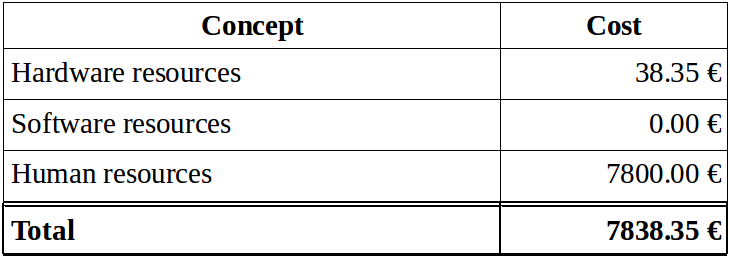
\includegraphics[width=0.7\textwidth]{total_budget}
    \caption{Total budget}
    \label{fig:total_budget}
\end{figure}

\subsection{Budget control}

The budget estimation as its name says is an estimation, therefore is not rigid and 
prone to changes.

The tasks that are more susceptible to deviations from the planning are the ones related 
to software architecture and development. If at any point there is a substantial delay 
in the development, the software developer will need to be hired for extra hours, 
thus changing the budget. On the other hand, I am confident with the planning and 
I don't expect any big deviation from it.

\section{Sustainability}

In the following sections I'll discuss the different areas of the sustainability of 
the project. Said areas are: economical sustainability, social sustainability and 
environmental sustainability.

\subsection{Economical sustainability}

In this document we have assessed the various costs of the resources required for 
the completion of the project.

The project is, in its core, a tool for reducing the work for a game developer. Once 
the framework is done, any future adjustments or updates will most probably be linked 
to a new need for a feature of a future project. The framework has been designed to 
be easily extended so the cost of future extensions should not be highly affected 
by the fact that they are extensions of the framework.

The cost of the project is relatively low and, although was not thought to be directly 
profitable, it will most probably be amortized when developing games with it, as it 
reduces the development time of video-games.

The service that this project will offer to its user could also be obtained from all 
the other game engine and frameworks that already exist in the market and open-source 
repositories. What this project offers is a lower level solution for those users that 
want to hand-craft their game from scratch.

\subsection{Social sustainability}

Nowadays, there is a high interest in game development. The video-game industry has 
grown a lot and many small studios have appeared. There have also appeared a set of 
full, free game-engines that have allowed for those small studios, and even students, 
to rapidly produce fully fleshed out products.

In this context, where these game-engines abstract all the inner systems from the 
user, some people may find they've lost control or that they want to learn the insides 
of a game. This is where this projects comes in. It offers the bare minimum systems 
for a game to be: a main loop, an actor pool with behaviors and a extension system 
to allow the user of the framework to extend it however they want, using any technology 
they want.

The scope of this project doesn't just involve the main framework, but also a multimedia 
plug-in for it. Any future user of the product will see the implementation time of 
their game reduced by just needing to focus on the gameplay systems. Therefore, improving 
the life of the game developer using it.

\subsection{Environmental sustainability}

The resources required for this project are listed in the Budget estimation section 
of this document.

During the development of this project the only resource that will consume energy 
will be the Laptop PC. Assuming it is connected all the time to an electricity source 
and the charger consuming around 60W, through all the project it will consume approximately 
13kWh, which is roughly equivalent to 3,9 kg of CO2\cite{CO2}. It is not a high amount 
of energy and may be reused by taking advantage of the laptop's battery.

\subsection{Sustainability table}

Considering the contents of this document, I've come up with the following table:

\begin{figure}[H]
    \centering
    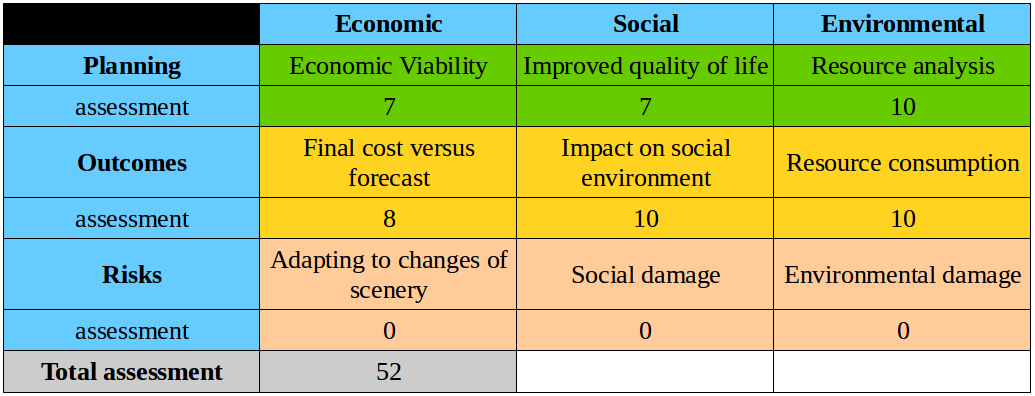
\includegraphics[width=\textwidth]{sustainability_table}
    \caption{Sustainability table}
    \label{fig:sustainability_table}
\end{figure}



\chapter{Conclusions}\label{ch:conclusions}

It has been a lot of work but I have learned more about the problems of implementing, 
not a game, but the scaffolding on top of which games are made.

Some features I've had to leave outside of the project due to time constraints and 
those were tough decisions I had to make in order to have a stable and functional product by 
the end.

Throughout the development, I managed to get feedback from some colleagues and my project's 
director, Guillem Godoy, and I've taken their views in the implementation so that 
the framework was as simple to use as possible.

In the end, I am satisfied with the current status of the project. The objectives were 
accomplished and exceeded and I feel the architecture makes it easier for developers 
to make games and learn by extending the framework using any preferred technology;
or just make a game using the MOGL plugin and focus on the game design and mechanics.

\chapter{Thanks}\label{ch:thanks}

Thank you all for your support.


\printbibliography

\chapter{Appendix}
\end{document}
